	\chapter{HTML Widgets}
        \section{Introduction}
	
	The ability to display statistical data is important in visualizing the information that is generated in scientific studies and research.
        Although \texttt{R} provides a method for visualizing data using graphs and plots, it is often challenging to represent demographic data.
        \texttt{htmlwidgets}, especially the \texttt{leaflet} package, is designed to address this concern.
        Furthermore, \texttt{leaflet} and any other \texttt{htmlwidgets} package can be integrated with \texttt{shiny} to produce a web application that fluidly portrays pertinent information.
	
	\section{Installation}
	
	The following code can be used to install the libraries that will be used in the demonstrations that follow.
	
        \begin{lstlisting}
                > install.packages("shiny")
                > install.packages("leaflet")
        \end{lstlisting}
	
	If the installation results in warnings about the \texttt{R} version you are using, please consider updating for the latest functionality.
	
	The installation, usage, and functionality of \texttt{ShinyApp} is expanded upon separately in another chapter of this R manual. Please consult that section of the book before continuing with the demonstrations outlined in this chapter. Although \texttt{leaflet} can be used in R without \texttt{ShinyApp} integration, the accessibility and functionality of these widgets is best used as a Web application.
	
	\section{Leaflet}
	
	Leaflet is one of the most popular open-source JavaScript libraries for interactive maps.
        It is used by websites ranging from The New York Times and The Washington Post to GitHub and Flickr, as well as GIS specialists like OpenStreetMap, Mapbox, and CartoDB \cite{leaflet}.
        The Leaflet libraries have been integrated fluidly into a R widget package form. We will learn the basics about this widget by creating some simple demonstrations.
	
	\subsection{Leaflet Demonstration 1 - A Simple Map}
	
	We can develop a simple user interface for our \texttt{ShinyApp} integration.
        Include a title panel, and create a sidebar layout.
        For this demonstration, we will simply have two numeric input controls that allow the user to enter the latitude and longitude.
        Our \texttt{ShinyApp} server will automatically render the new position onto the Leaflet map.
	
        \begin{lstlisting}
        library(shiny)
        library(leaflet)
        
        ### USER INTERFACE ###
        
        ui <- fluidPage(
                # Title of the ShinyApp
                titlePanel("Leaflet Demonstration 1"),
                # A layout with a sidebar
                sidebarLayout(
                        # Content of the sidebar panel
                        sidebarPanel(
                                # Two input controls
                                numericInput("lat", "Latitude:", min=-90, max=90, value=44.366002, step=0.001),
                                numericInput("lon", "Longitude:", min=-180, max=180, value=-68.196409, step=0.001)
                        ),
                        # Content of the main panel
                        mainPanel(
                                # The leaflet widget UI
                                leafletOutput("map")
                        )
                )
        )
        \end{lstlisting}

	For the server-side logic, we simply render the leaflet using a reactive system so that every time the latitude or longitude is updated, the map renders itself again. We generate a \texttt{leaflet()} object and assign it certain attributes from functions that are provided by the \texttt{leaflet} package. The \texttt{addTiles()} command ensures that the map will use the default map tiles that are provided in the package. The \texttt{addMarkers()} command adds a marker on the map that points to the location that has been chosen. This command also supports multiple markers in one command.
	
        \begin{lstlisting}
        ### SERVER LOGIC ###
        
        server <- function(input, output) {
                # Set the output map using a rendering function
                output$map <- renderLeaflet({
                        # The leaflet object
                        leaflet() %>%
                                addTiles() %>%
                                addMarkers(lng=input$lon, lat=input$lat, popup="The Location")
                })
        }
        \end{lstlisting}	
	
	Finally, we run the server using the \texttt{shinyApp()} command.
        We pass both the user interface and the server logic as arguments.
        The server will run on a local address, such as \texttt{http://127.0.0.1:7591}. 
	
        \begin{lstlisting}
        shinyApp(ui=ui, server=server)
        \end{lstlisting}

	Running the server produces an interactive map with a marker at the location that has been specified with the latitude and longitude in the sidebar.
        By changing the values, we can change the location reactively.
        Furthermore, we can zoom in and out of the map using the scroll function or the buttons provided on the map.
        Finally, we can also drag around the map by clicking inside the map control.
	
	\begin{figure}[htbp!]
		\centering
		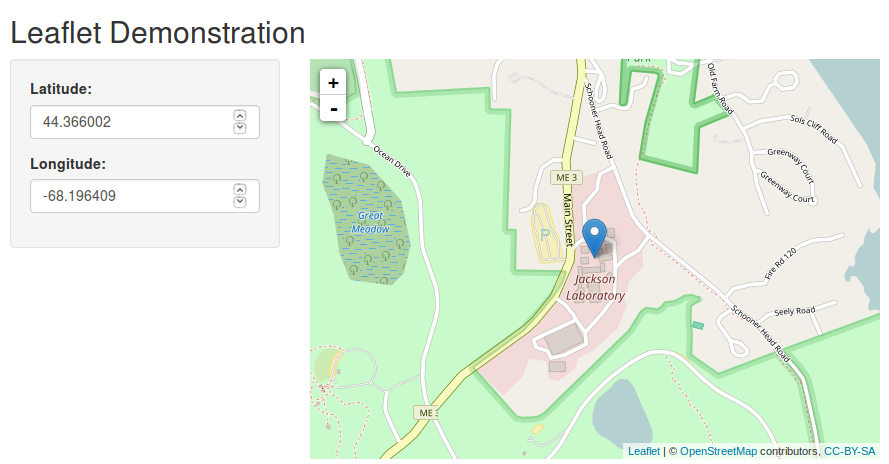
\includegraphics[width=12cm]{pictures/html/htmlwidgets-image-1.png}
		\caption{The Result of our First Demonstration}
	\end{figure}

	\subsection{Leaflet Demonstration 2 - Map Tiles}
	
	In this section, we will explore the different views and tiles that are provided by third-party developers.
        We will only be changing the part of the code that renders the \texttt{leaflet()} in the server logic.
        The \texttt{setView()} command allows us to choose the location of the initial view and the level of zoom.
	
        \begin{lstlisting}
        # Stamen.Toner
        output$map <- renderLeaflet({
                leaflet() %>%
                        addProviderTiles("Stamen.Toner") %>%
                        setView(lng=-71.0589, lat=42.3601, zoom=12)
        })
        # CartoDB.Positron
        output$map <- renderLeaflet({
                leaflet() %>%
                        addProviderTiles("CartoDB.Positron") %>%
                        setView(lng=-71.0589, lat=42.3601, zoom=12)
        })
        \end{lstlisting}

	\begin{figure}[htbp!]
		\centering
		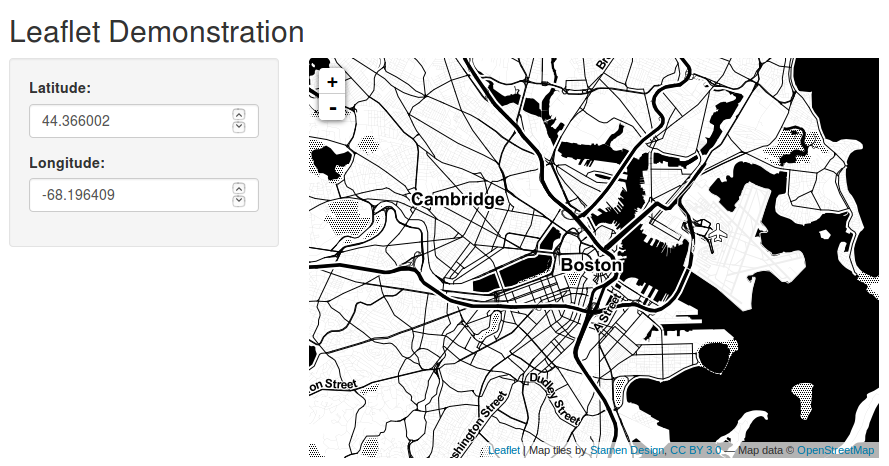
\includegraphics[width=.5\textwidth]{pictures/html/htmlwidgets-image-2.png}
		\caption{The Toner Tiles}
	\end{figure}

	\begin{figure}[htbp!]
		\caption{The Positron Tiles}
		\centering
		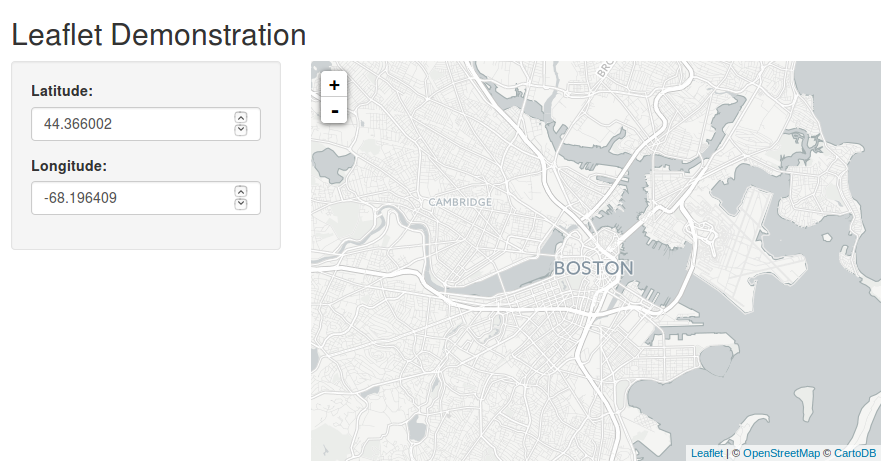
\includegraphics[width=.5\textwidth]{pictures/html/htmlwidgets-image-3.png}
	\end{figure}

	\subsubsection{Web Map Service Tiles}
	
	We can use interesting commands to overlay the graphics from other web map services onto our tiles.
        For example, we will create a map that shows the intensity of precipitation by using the \texttt{addWMSTiles()} command.
	
        \begin{lstlisting}
        output$map <- renderLeaflet({
                leaflet() %>%
                        addTiles() %>%
                        setView(-93.65, 42.0285, zoom=4) %>%
                        addWMSTiles(
                                "http://mesonet.agron.iastate.edu/cgi-bin/wms/nexrad/n0r.cgi",
                                layers = "nexrad-n0r-900913",
                                options = WMSTileOptions(format = "image/png", transparent = TRUE),
                                attribution = "Weather data Copyright 2012 IEM Nexrad"
                        )
        })
        \end{lstlisting}

	\begin{figure}[htbp!]
		\centering
		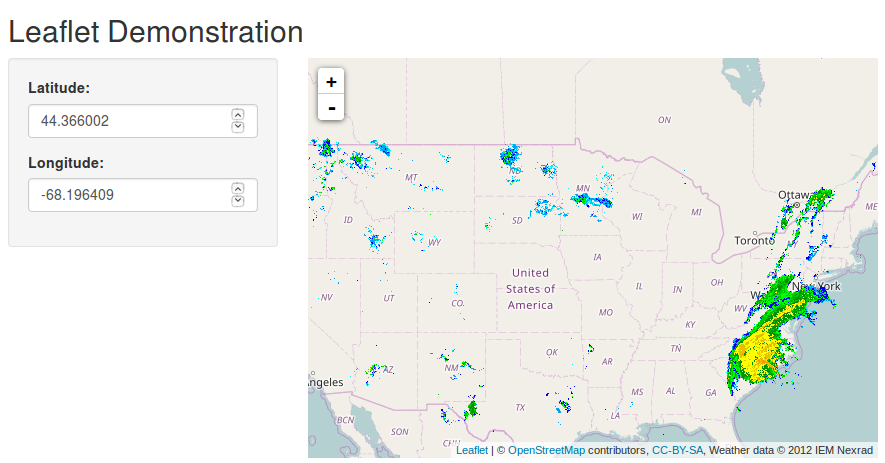
\includegraphics[width=.5\textwidth]{pictures/html/htmlwidgets-image-4.png}
		\caption{The Weather Data for Precipitation}
	\end{figure}

	\subsection{Leaflet Student Demonstration - Markers}
	
	One of the most important functions of this widget, and this chapter in general, is the ability to correctly visualize data.
        To accomplish this, we utilize markers, which are inconsequential to visualizing data on maps.
        We will use population data from some major cities in America and use different markers to visualize the data.
	
	\noindent\textbf{Student Prompt: } Use the following code that provides population data to develop a map that accurately demonstrates the size of each city mentioned in the dataset.
		
        \begin{lstlisting}
                population <- read.csv(textConnection(
                "City,Population,Lat,Lon,
                        Nashville,678889,36.1627,-86.7816
                        Asheville,87236,35.5951,-82.5515
                        Portland,609456,45.5231,-122.6765
                        Denver,649495,39.7392,-104.9903
                        Kansas City,467007,39.0997,-94.5786
                        Seattle,652405,47.6062,-122.3321
                        New York City,8406000,40.7128,-74.0059"
                ), header=TRUE)
        \end{lstlisting}

	\noindent\textbf{Solution}
	
	In general, after using the documentation found on the web, most students will create a solution as follows:

        \begin{lstlisting}
        server <- function(input, output) {
                
                output$map <- renderLeaflet({
                        leaflet(data=population) %>%
                                addTiles() %>%
                                addMarkers(~Lon, ~Lat, popup=~paste(sep="<br/>", paste(sep="", "<b>", as.character(City), "</b>"), as.character(Population)))
                })
        }
        \end{lstlisting}

	The code will generate the following maps.
        Unfortunately, this type of visualization, while informative about the location of every city, does not help visualize any part of the population in every location.
        We will instead try to create a visual representation of the population in every location by generating circles with an area proportional to the population of the city.
	
	\begin{figure}[htbp!]
		\centering
		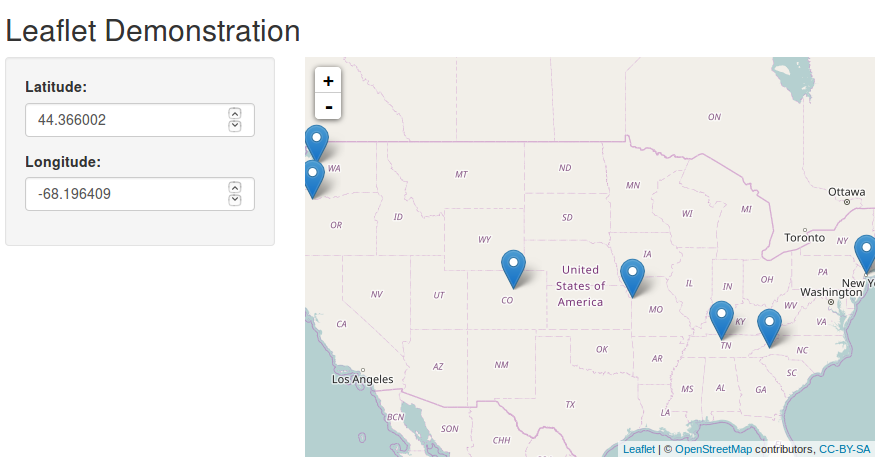
\includegraphics[width=12cm]{pictures/html/htmlwidgets-image-5.png}
		\caption{The Markers Placed at Every Location}
	\end{figure}

	The \texttt{addCircleMarkers()} allows us to add circles that have custom properties depending on the data point.
        We will use the \texttt{radius} attribute to make the circle larger or smaller depending on the population of the city.
	
        \begin{lstlisting}
        output$map <- renderLeaflet({
                leaflet(data=population) %>%
                        addTiles() %>%
                        addCircleMarkers(~Lon, ~Lat, popup=~paste(sep="<br/>", paste(sep="", "<b>", as.character(City), "</b>"), as.character(Population)), radius=~sqrt(Population/1000))
        })
        \end{lstlisting}
	
	\begin{figure}[htbp!]
		\centering
		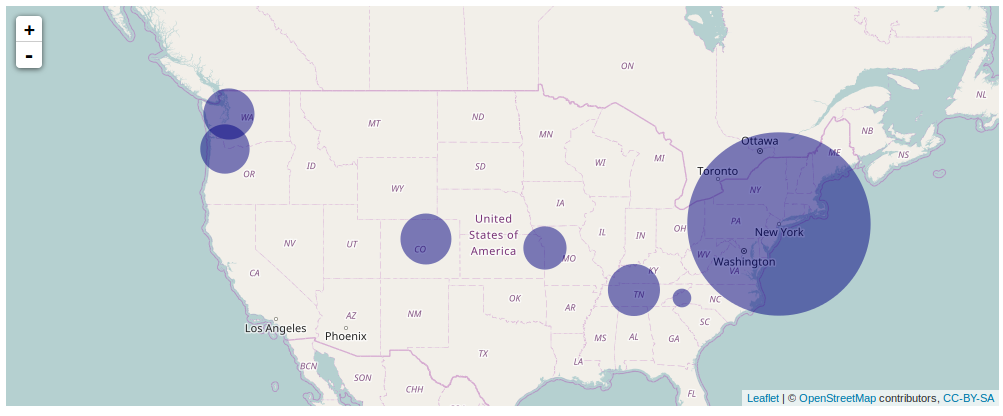
\includegraphics[width=.5\textwidth]{pictures/html/htmlwidgets-image-6.png}
		\caption{The Markers Placed at Every Location}
	\end{figure}
